\documentclass[main.tex]{subfiles}
\begin{document}
	然后单击 Spyder 下面的 Launch 就会打开 Spyder。单击 Jupyter 下面的 Launch 就会打开 Spyder
打开 Spyder
\begin{figure}[h]
	\centering
	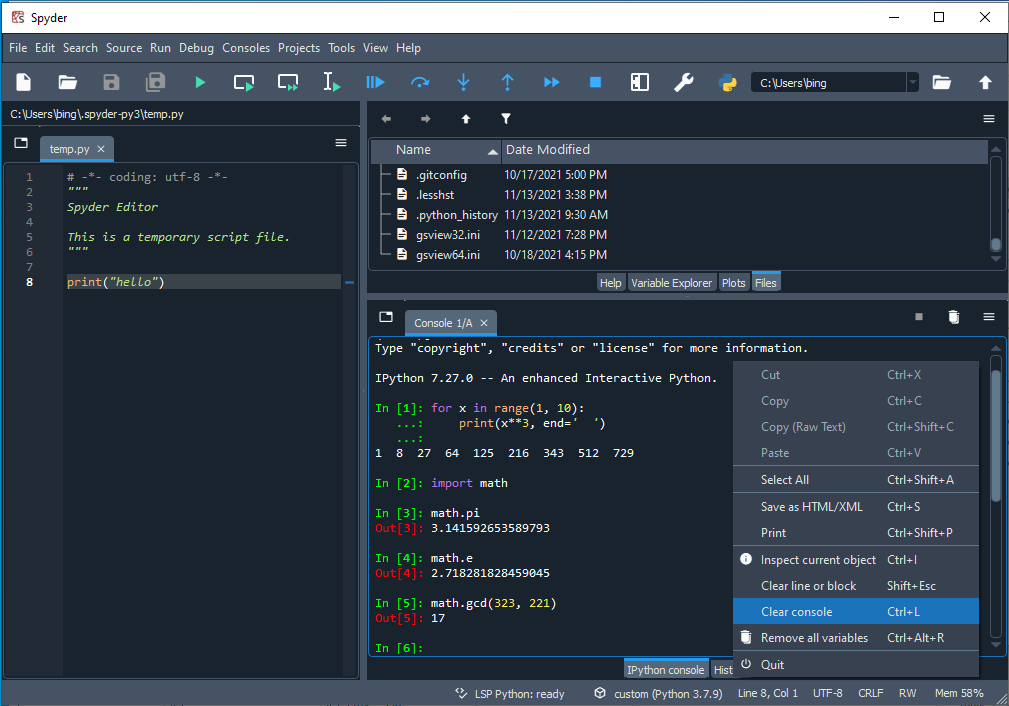
\includegraphics[width=1.0\textwidth]{png/spyder_ide.png}
	\caption{Spyder IDE}
	\label{fig:2.3.1}
\end{figure}


the Specifying Colors tutorial;
the matplotlib.colors API;
the Color Demo.


\begin{small}
\begin{spacing}{0.8}
\begin{lstlisting}[language=Python]
  1  import re
  2  
  3  x = "100以内有25个质数。不实际计算的话,其中51和91很容易被误判为是质数。"
  4  x = re.sub("质数", "素数", x)
  5  x = x.replace("其中", '')
  6  print(x)
\end{lstlisting}
\end{spacing}

\end{small}

\end{document} 
